\documentclass[main.tex]{subfiles}
\begin{document}
\glsresetall

\section{Introduction}

During the commissioning phase of the \gls{lst} 1, one of the objectives is to test the uniformity of the camera and perform the necessary adjustments to ensure it. The non-uniformity along all the pixels of the camera translates in some pixels or modules to be more probable to trigger than others, biasing the results of the data analysis shown in chapter \ref{cap:LST1}. To have an idea of the uniformity of the camera during the three Crab campaigns, and spot possible problems in the data, the distribution of the centroids of the Hillas ellipses in the camera has been plotted for each day of observation. This way, anisotropies can be observed, pointing to pixels that are triggered with a different frequency than the mean.

\section{Distribution of centroids of Hillas ellipses for standard analysis}

In this setion, the centroids calculated using the standard \gls{lst}1 analysis, as described in section \ref{sec:anachain}, are shown in pictures \ref{fig:1st-crab-campaign-cog}, \ref{fig:2nd-crab-campaign-cog} and \ref{fig:3rd-crab-campaign-cog}.

\begin{figure}[h!]
  \begin{subfigure}{0.45\textwidth}
    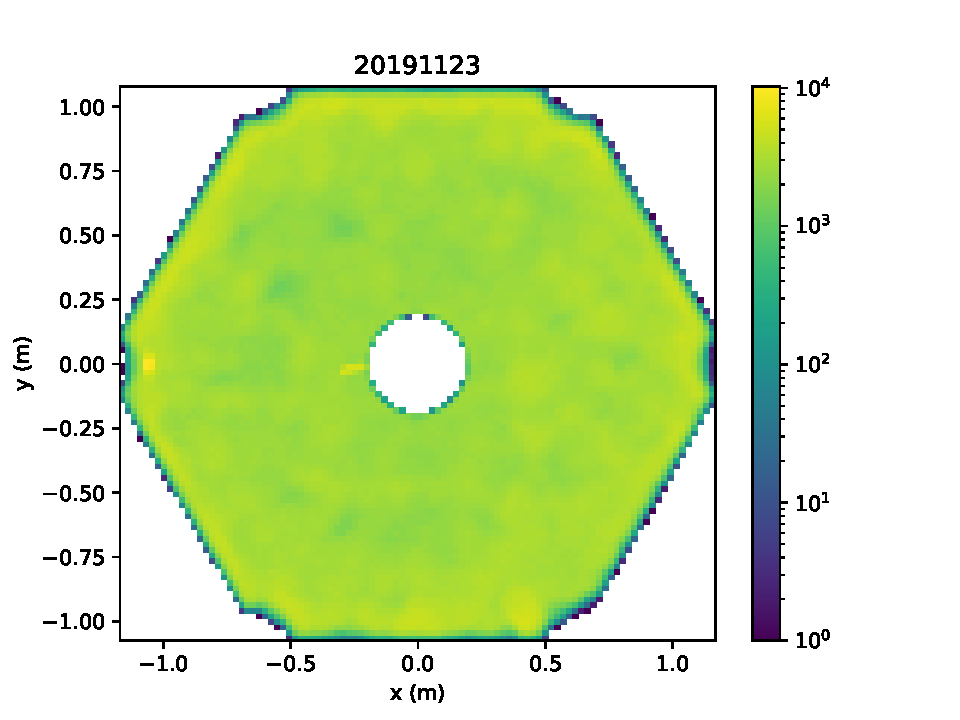
\includegraphics[width=\linewidth]{{Pictures/20191123_sizecut100}.pdf}
    \caption{\small 23/11/2019} \label{fig:1st-cog-a}
  \end{subfigure}
  \begin{subfigure}{0.45\textwidth}
    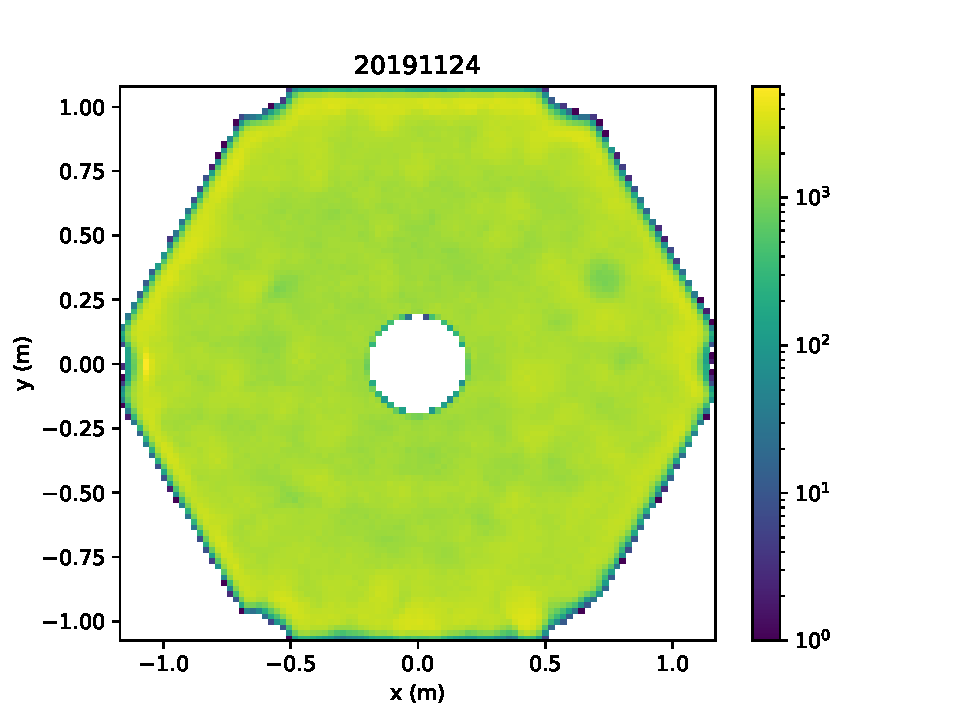
\includegraphics[width=\linewidth]{{Pictures/20191124_sizecut100}.pdf}
    \caption{\small 24/11/2019} \label{fig:1st-cog-b}
  \end{subfigure} \\
  \begin{subfigure}{0.45\textwidth}
    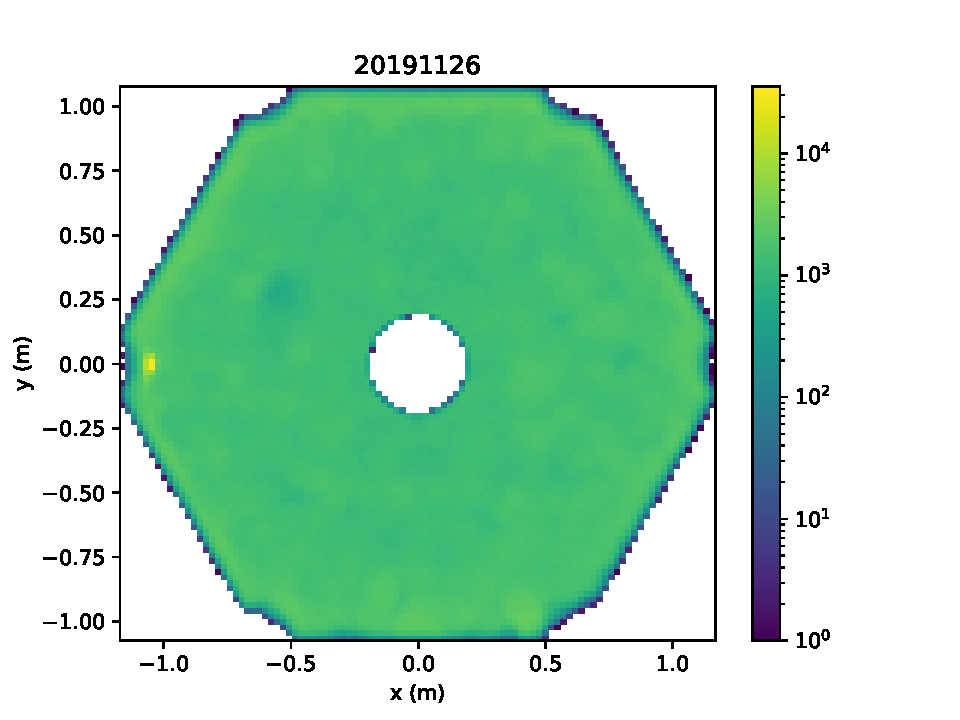
\includegraphics[width=\linewidth]{{Pictures/20191126_sizecut100}.pdf}
    \caption{\small 26/11/2019} \label{fig:1st-cog-c}
  \end{subfigure}
  \begin{subfigure}{0.45\textwidth}
    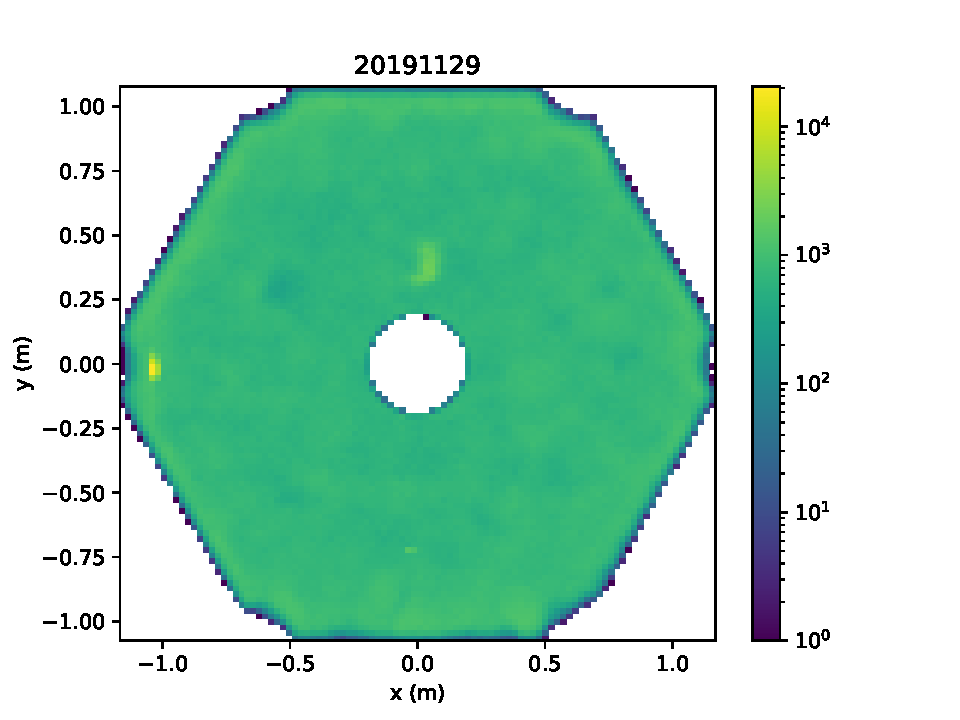
\includegraphics[width=\linewidth]{{Pictures/20191129_sizecut100}.pdf}
    \caption{\small 29/11/2019} \label{fig:1st-cog-d}
  \end{subfigure}
  \caption{Distribution of the positions in the camera of the center of gravity of Hillas ellipses for the data taken during the different days of the First Crab Campaign.}\label{fig:1st-crab-campaign-cog}
\end{figure}


\begin{figure}[h!]
  \begin{subfigure}{0.45\textwidth}
    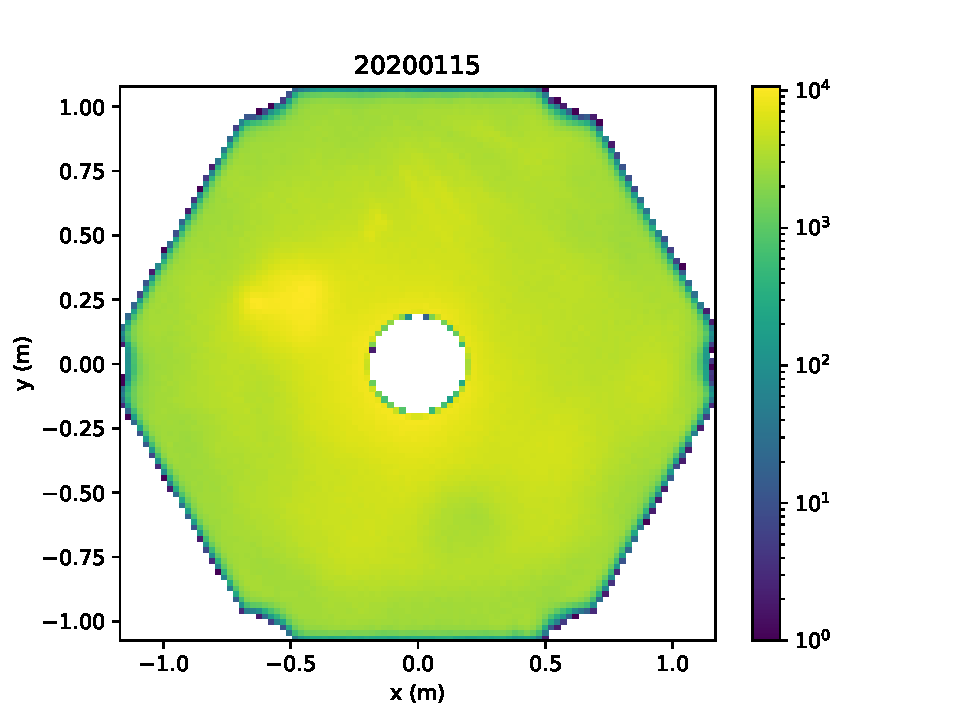
\includegraphics[width=\linewidth]{{Pictures/20200115_sizecut100}.pdf}
    \caption{\small 15/01/2020} \label{fig:2nd-cog-a}
  \end{subfigure}
  \begin{subfigure}{0.45\textwidth}
    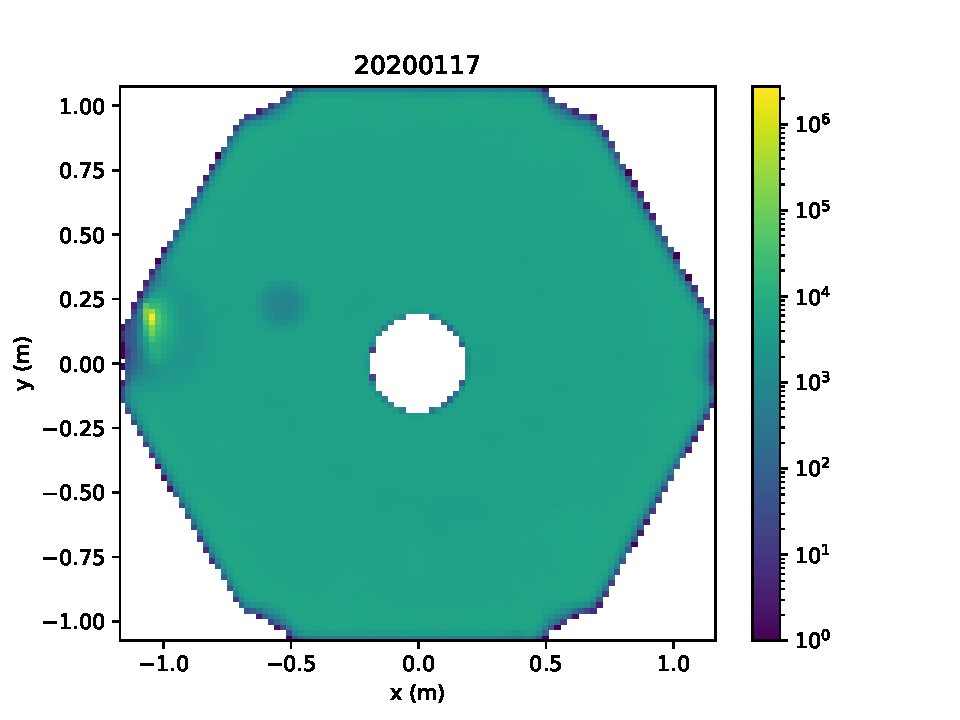
\includegraphics[width=\linewidth]{{Pictures/20200117_sizecut100}.pdf}
    \caption{\small 17/01/2020} \label{fig:2nd-cog-b}
  \end{subfigure} \\
  \begin{subfigure}{0.45\textwidth}
    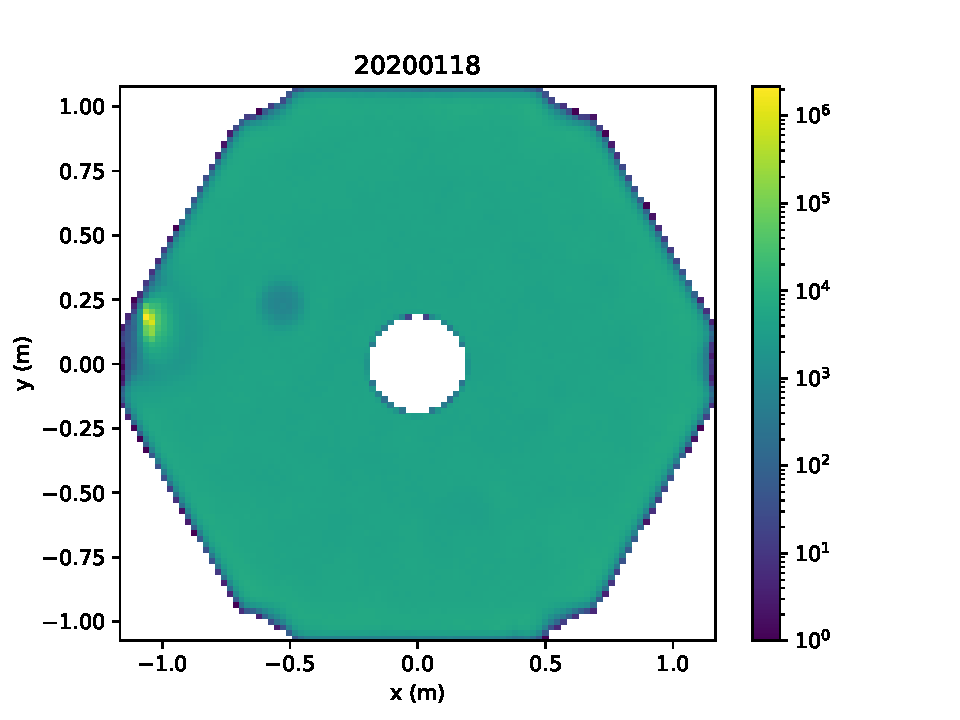
\includegraphics[width=\linewidth]{{Pictures/20200118_sizecut100}.pdf}
    \caption{\small 18/01/2020} \label{fig:2nd-cog-c}
  \end{subfigure}
  \begin{subfigure}{0.45\textwidth}
    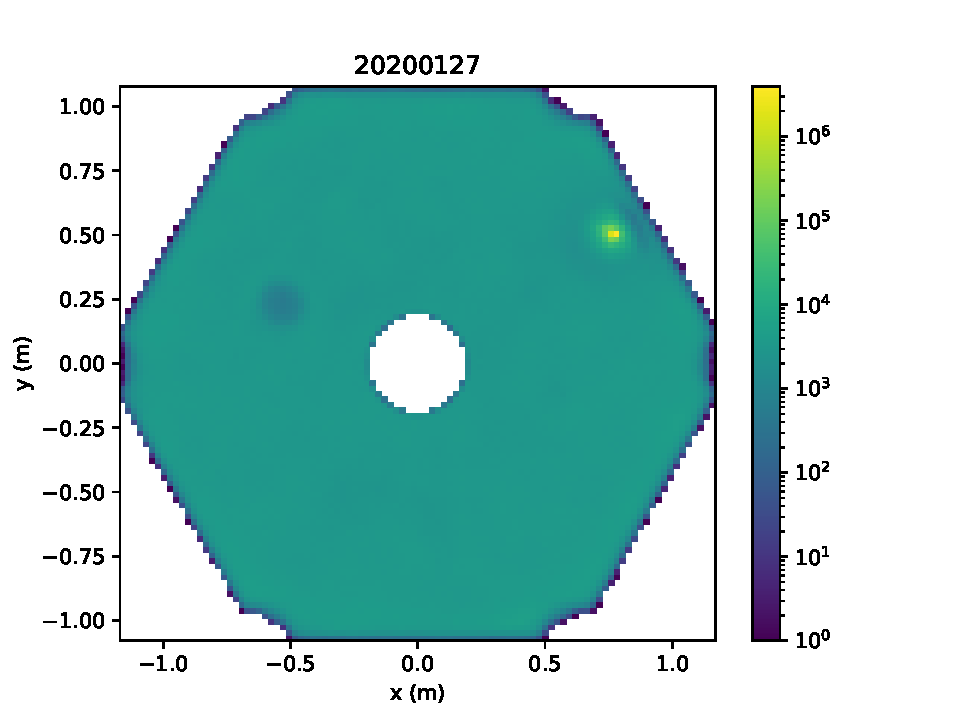
\includegraphics[width=\linewidth]{{Pictures/20200127_sizecut100}.pdf}
    \caption{\small 27/01/2020} \label{fig:2nd-cog-d}
  \end{subfigure} \\
  \begin{subfigure}{0.45\textwidth}
    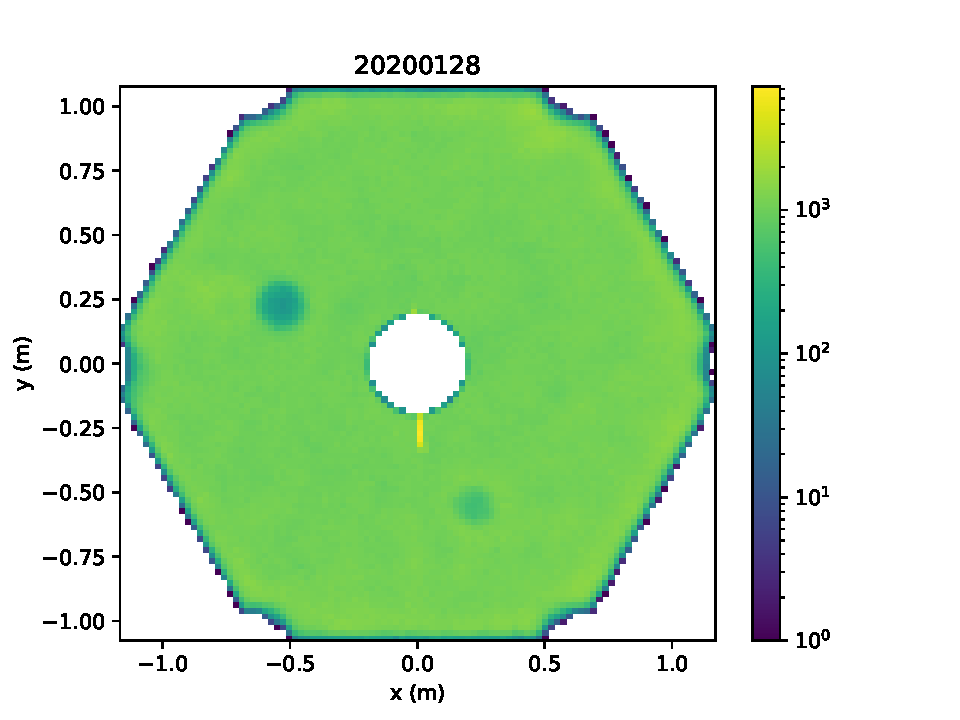
\includegraphics[width=\linewidth]{{Pictures/20200128_sizecut100}.pdf}
    \caption{\small 28/01/2020} \label{fig:2nd-cog-c}
  \end{subfigure}
  \caption{Distribution of the positions in the camera of the center of gravity of Hillas ellipses for the data taken during the different days of the Second Crab Campaign. \label{fig:2nd-crab-campaign-cog}}
\end{figure}


\begin{figure}[h!]
  \begin{subfigure}{0.45\textwidth}
    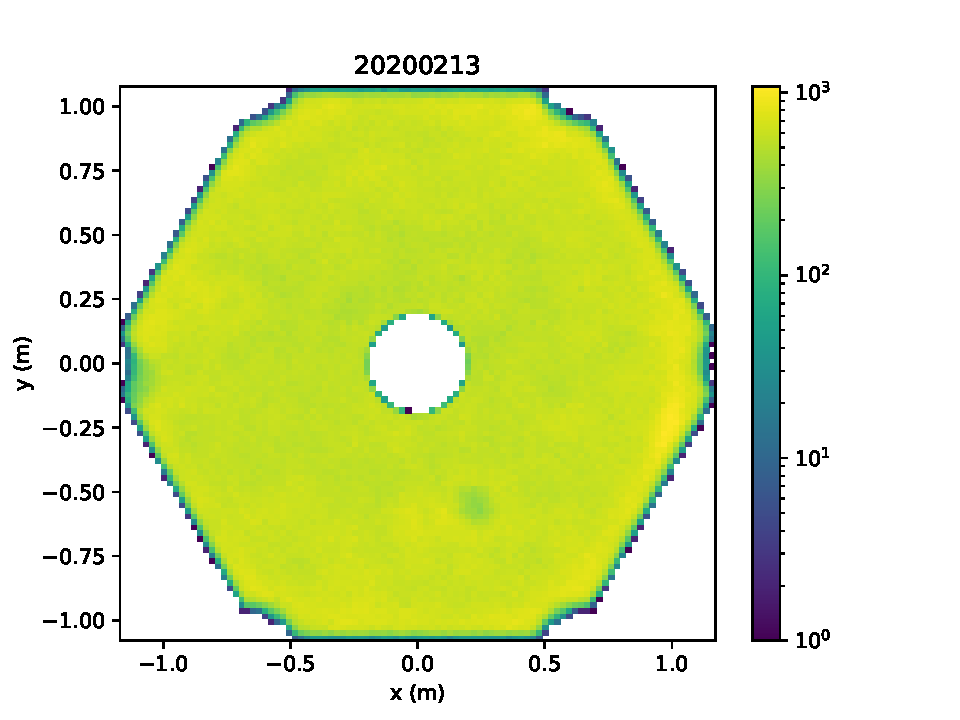
\includegraphics[width=\linewidth]{{Pictures/20200213_sizecut100}.pdf}
    \caption{\small 13/02/2020} \label{fig:3rd-cog-a}
  \end{subfigure}
  \begin{subfigure}{0.45\textwidth}
    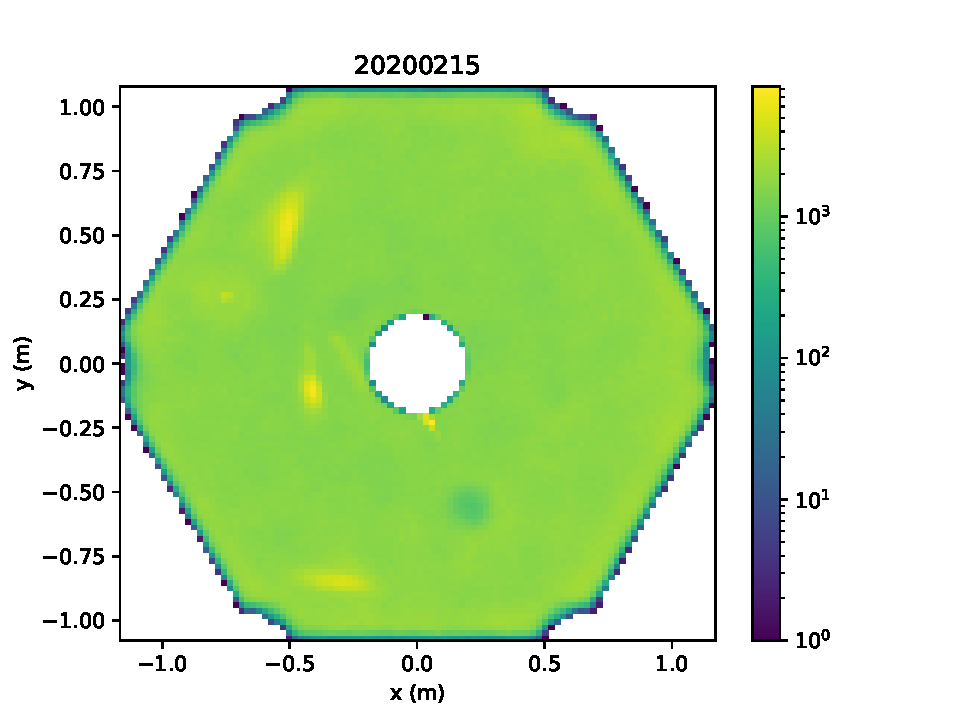
\includegraphics[width=\linewidth]{{Pictures/20200215_sizecut100}.pdf}
    \caption{\small 15/02/2020} \label{fig:3rd-cog-b}
  \end{subfigure} \\
  \begin{subfigure}{0.45\textwidth}
    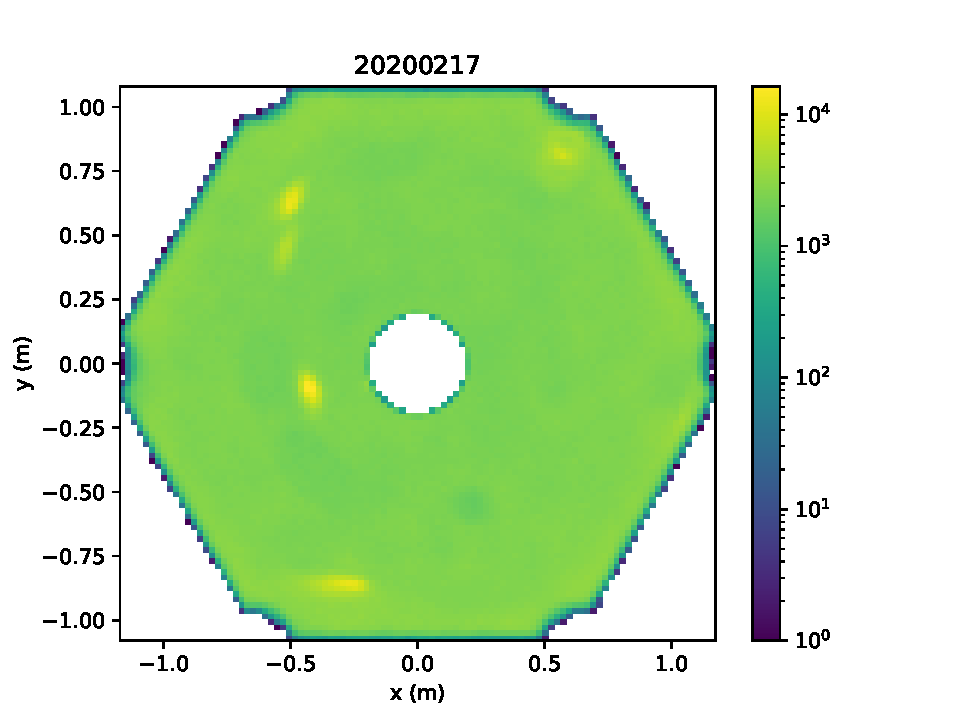
\includegraphics[width=\linewidth]{{Pictures/20200217_sizecut100}.pdf}
    \caption{\small 17/02/2020} \label{fig:3rd-cog-c}
  \end{subfigure}
  \begin{subfigure}{0.45\textwidth}
    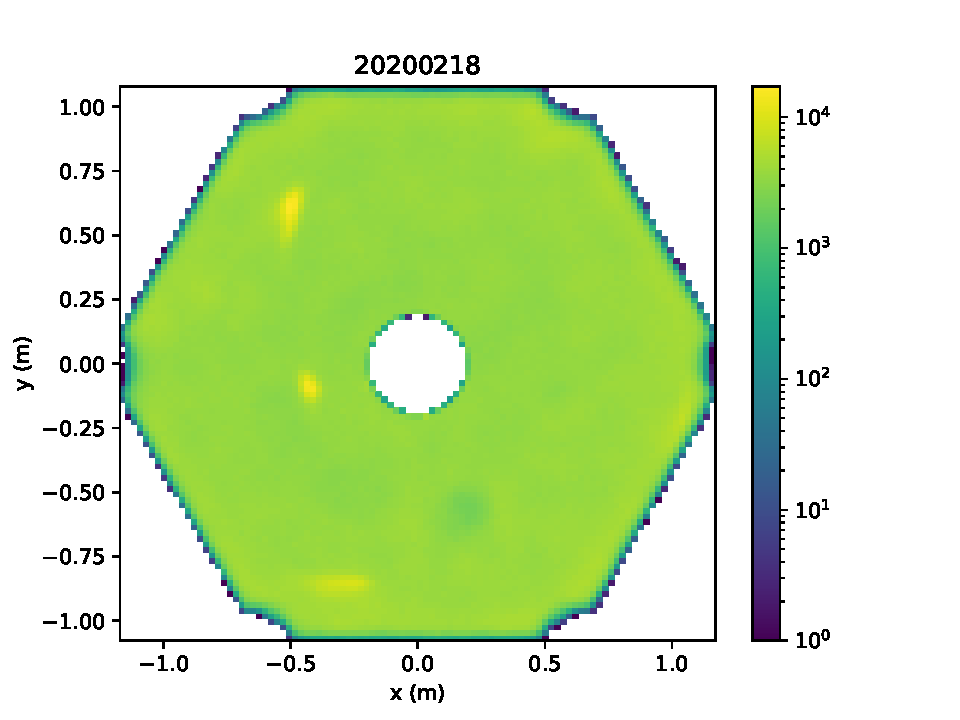
\includegraphics[width=\linewidth]{{Pictures/20200218_sizecut100}.pdf}
    \caption{\small 18/02/2020} \label{fig:3rd-cog-d}
  \end{subfigure} \\
  \begin{subfigure}{0.45\textwidth}
    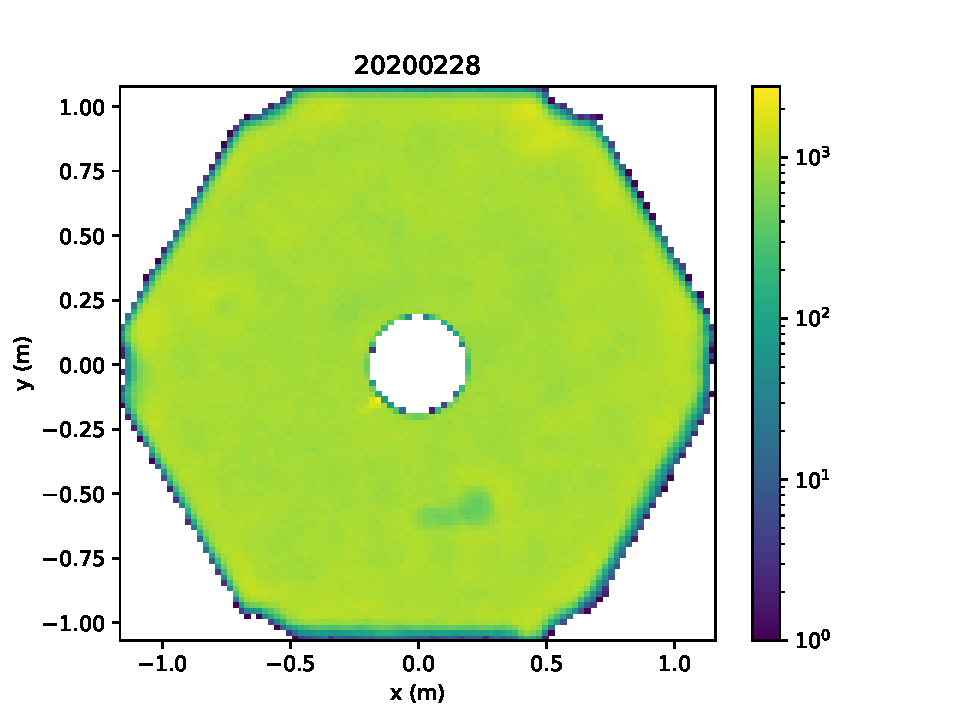
\includegraphics[width=\linewidth]{{Pictures/20200228_sizecut100}.pdf}
    \caption{\small 28/02/2020} \label{fig:3rd-cog-d}
  \end{subfigure}\\
  \caption{ Distribution of the positions in the camera of the center of gravity of Hillas ellipses for the data taken during the different days of the Third Crab Campaign.\label{fig:3rd-crab-campaign-cog}}
\end{figure}

\section{Distribution of centroids of Hillas ellipses for Expectation-Maximization analysis}


In this setion, the centroids calculated using the \gls{em} method for Hillas parameterization, as described in section \ref{sec:em}, are shown in pictures \ref{fig:em_1st-crab-campaign-cog}, \ref{fig:em_2nd-crab-campaign-cog} and \ref{fig:em_3rd-crab-campaign-cog}.

\begin{figure}[h!]
  \begin{subfigure}{0.45\textwidth}
    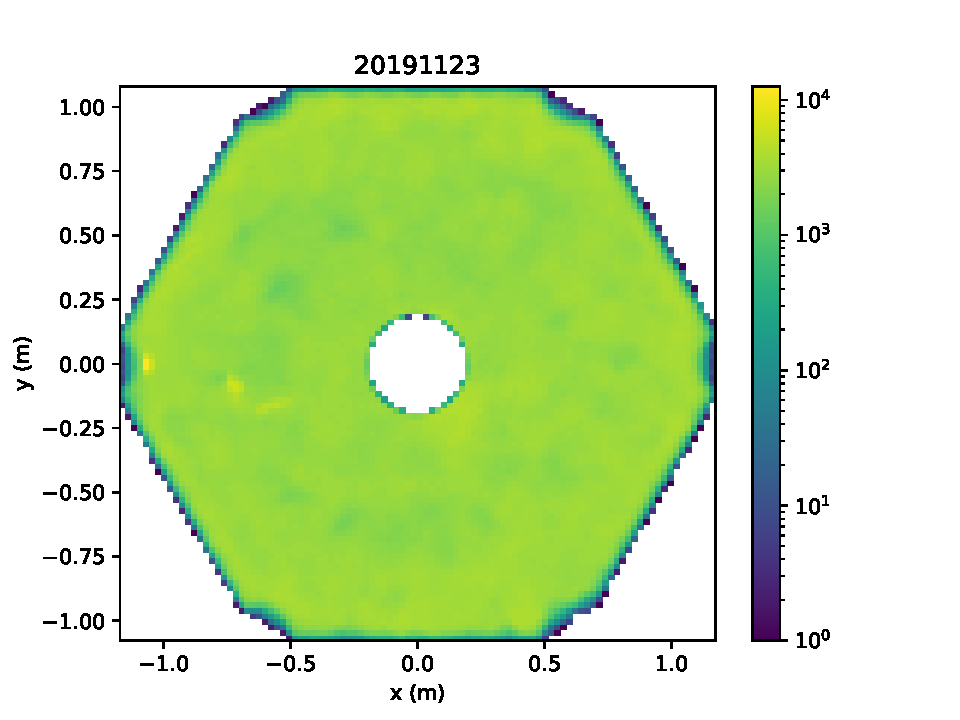
\includegraphics[width=\linewidth]{{Pictures/em_20191123_sizecut100}.pdf}
    \caption{\small 23/11/2019} \label{fig:1st-cog-a}
  \end{subfigure}
  \begin{subfigure}{0.45\textwidth}
    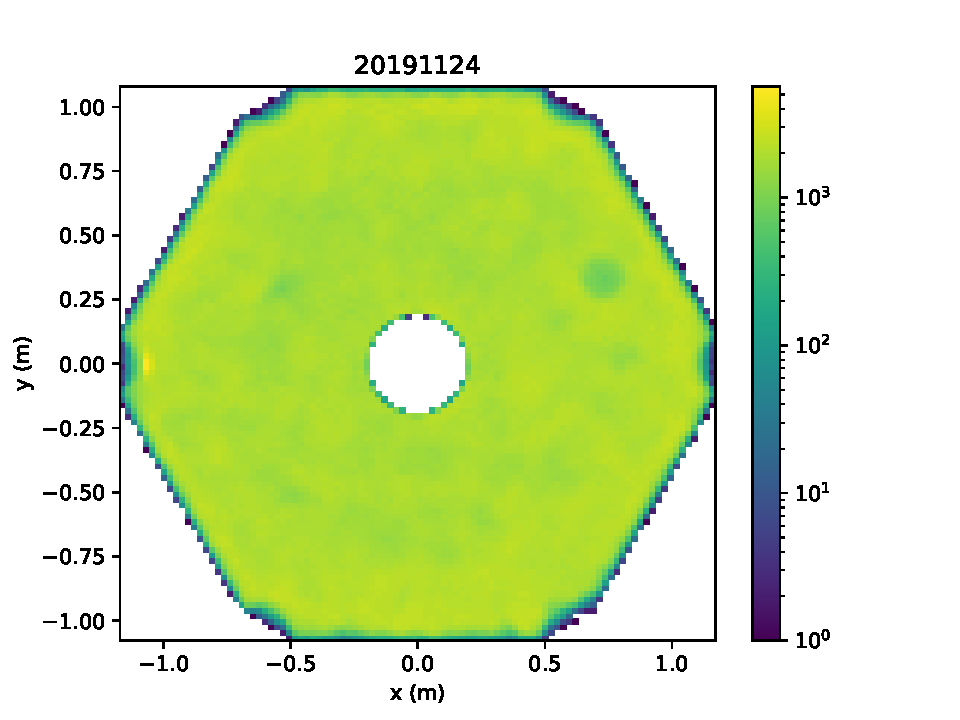
\includegraphics[width=\linewidth]{{Pictures/em_20191124_sizecut100}.pdf}
    \caption{\small 24/11/2019} \label{fig:1st-cog-b}
  \end{subfigure} \\
  \begin{subfigure}{0.45\textwidth}
    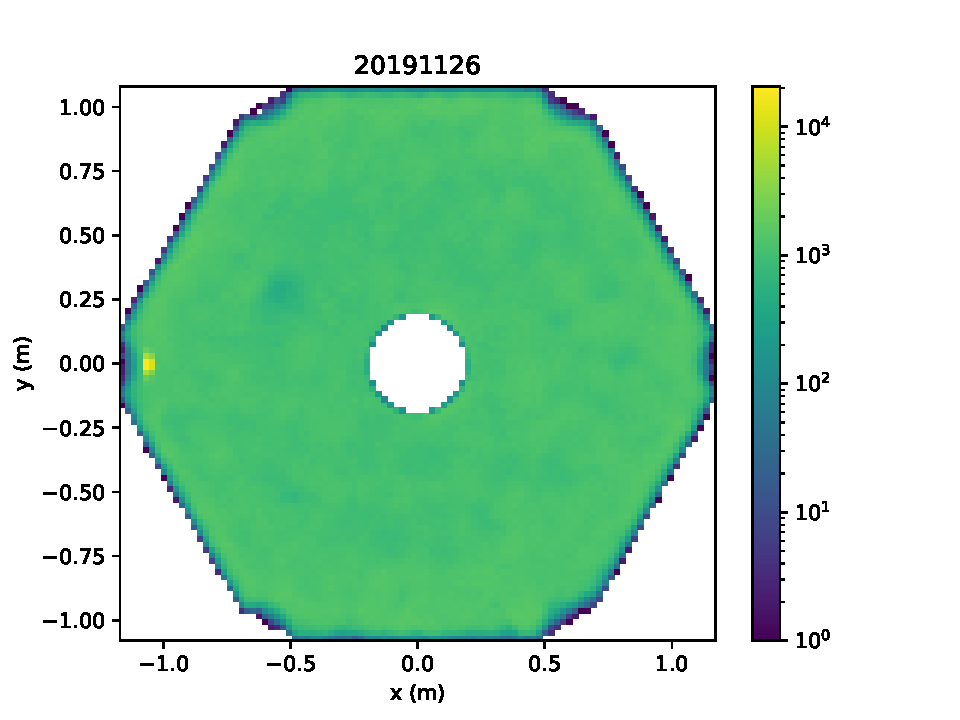
\includegraphics[width=\linewidth]{{Pictures/em_20191126_sizecut100}.pdf}
    \caption{\small 26/11/2019} \label{fig:1st-cog-c}
  \end{subfigure}
  \begin{subfigure}{0.45\textwidth}
    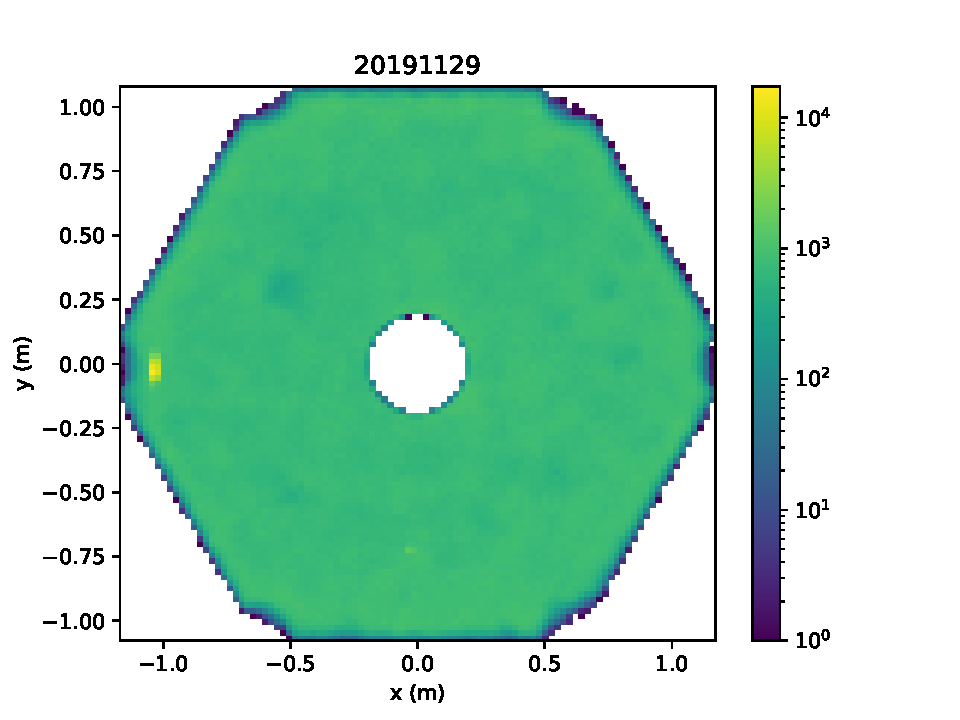
\includegraphics[width=\linewidth]{{Pictures/em_20191129_sizecut100}.pdf}
    \caption{\small 29/11/2019} \label{fig:1st-cog-d}
  \end{subfigure}
  \caption{Distribution of the positions in the camera of the center of gravity of Hillas ellipses for the data taken during the different days of the First Crab Campaign, using the \gls{em} method for Hillas parameterization.}\label{fig:em_1st-crab-campaign-cog}
\end{figure}


\begin{figure}[h!]
  \begin{subfigure}{0.45\textwidth}
    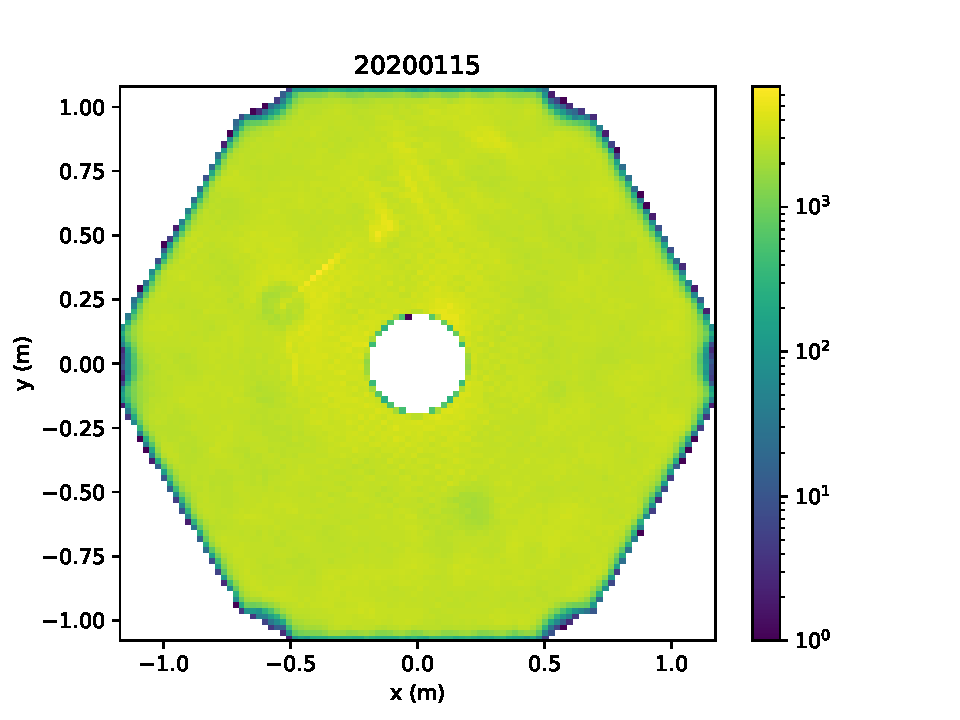
\includegraphics[width=\linewidth]{{Pictures/em_20200115_sizecut100}.pdf}
    \caption{\small 15/01/2020} \label{fig:2nd-cog-a}
  \end{subfigure}
  \begin{subfigure}{0.45\textwidth}
    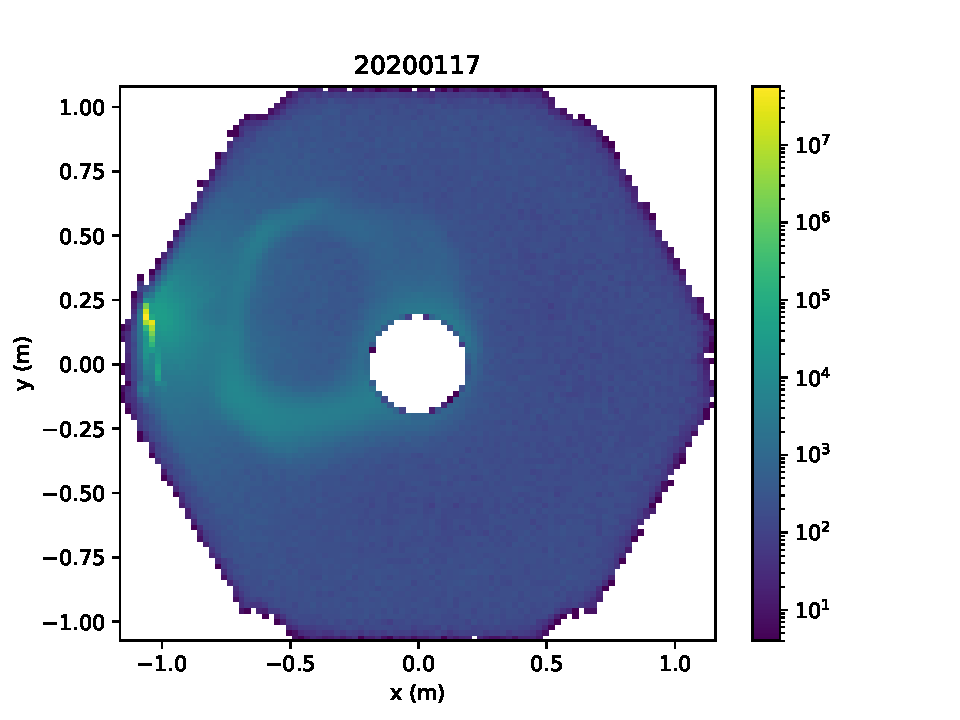
\includegraphics[width=\linewidth]{{Pictures/em_20200117_sizecut100}.pdf}
    \caption{\small 17/01/2020} \label{fig:2nd-cog-b}
  \end{subfigure} \\
  \begin{subfigure}{0.45\textwidth}
    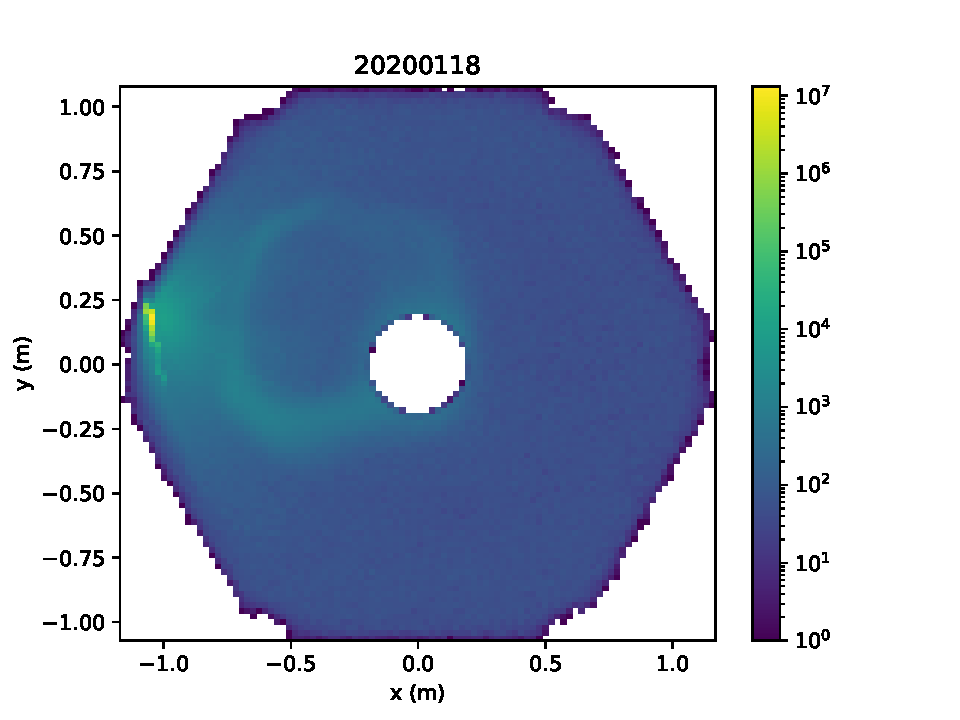
\includegraphics[width=\linewidth]{{Pictures/em_20200118_sizecut100}.pdf}
    \caption{\small 18/01/2020} \label{fig:2nd-cog-c}
  \end{subfigure}
  \begin{subfigure}{0.45\textwidth}
    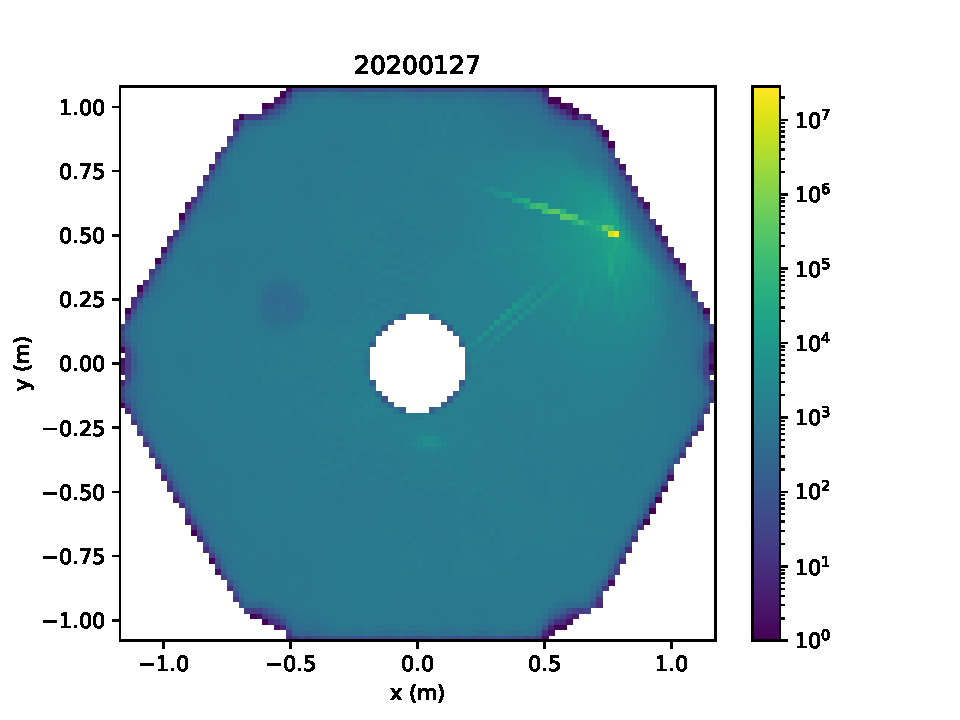
\includegraphics[width=\linewidth]{{Pictures/em_20200127_sizecut100}.pdf}
    \caption{\small 27/01/2020} \label{fig:2nd-cog-d}
  \end{subfigure} \\
  \begin{subfigure}{0.45\textwidth}
    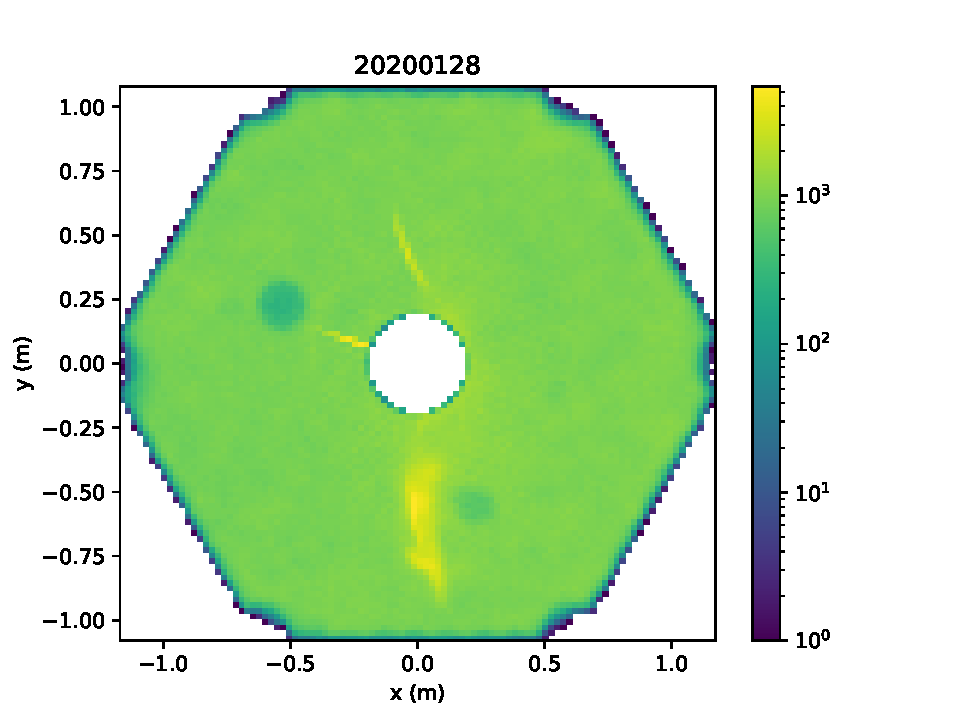
\includegraphics[width=\linewidth]{{Pictures/em_20200128_sizecut100}.pdf}
    \caption{\small 28/01/2020} \label{fig:2nd-cog-c}
  \end{subfigure}
  \caption{Distribution of the positions in the camera of the center of gravity of Hillas ellipses for the data taken during the different days of the Second Crab Campaign, using the \gls{em} method for Hillas parameterization. \label{fig:em_2nd-crab-campaign-cog}.}
\end{figure}

\begin{figure}[h!]
  \begin{subfigure}{0.45\textwidth}
    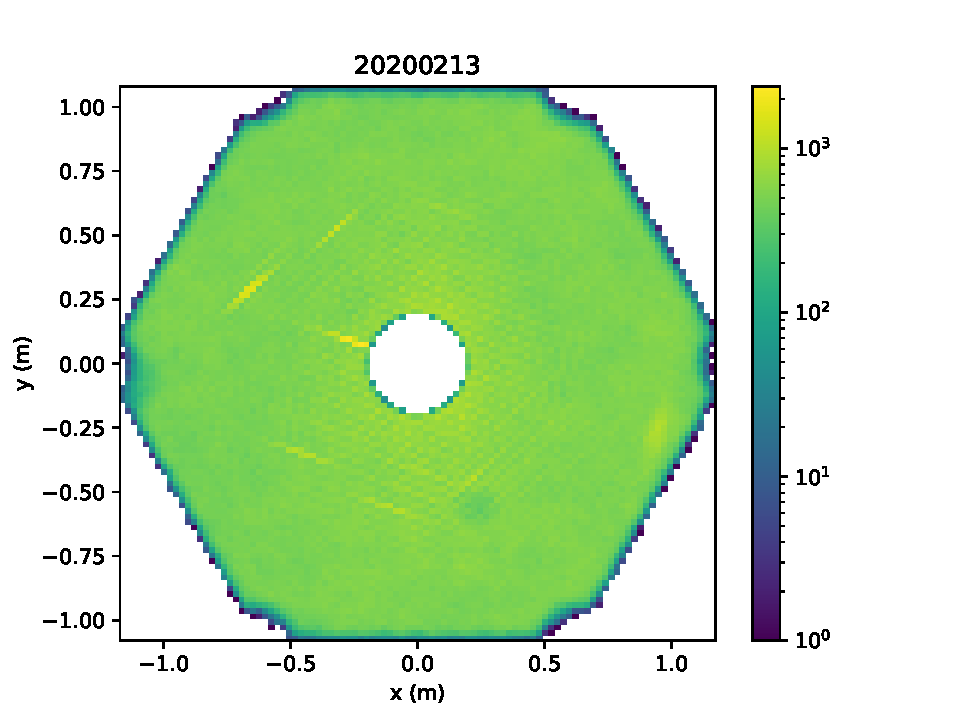
\includegraphics[width=\linewidth]{{Pictures/em_20200213_sizecut100}.pdf}
    \caption{\small 13/02/2020} \label{fig:3rd-cog-a}
  \end{subfigure}
  \begin{subfigure}{0.45\textwidth}
    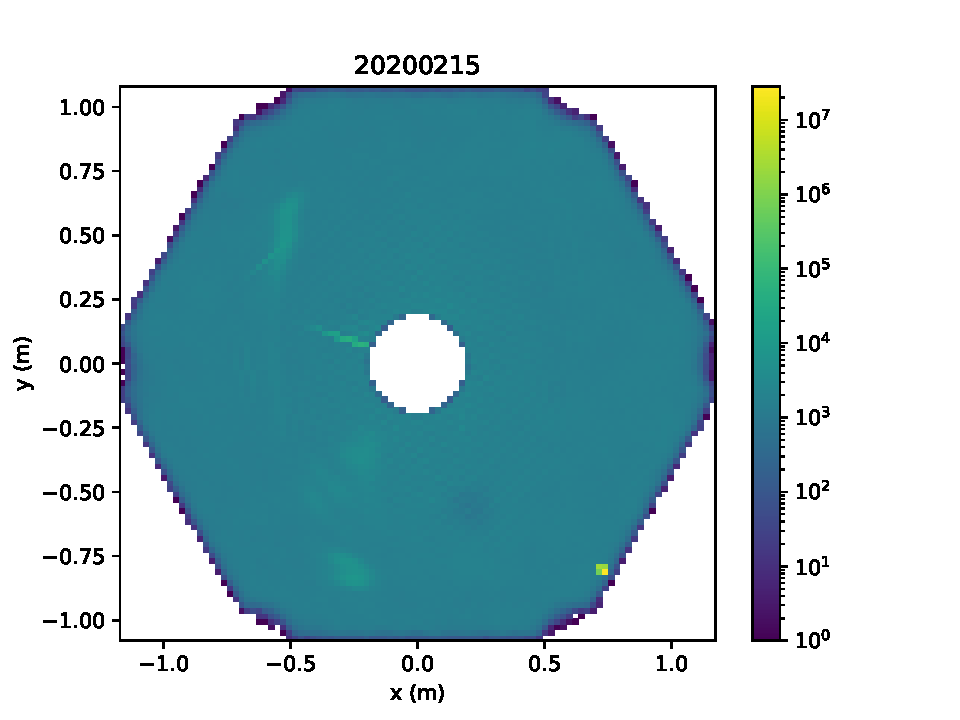
\includegraphics[width=\linewidth]{{Pictures/em_20200215_sizecut100}.pdf}
    \caption{\small 15/02/2020} \label{fig:3rd-cog-b}
  \end{subfigure} \\
  \begin{subfigure}{0.45\textwidth}
    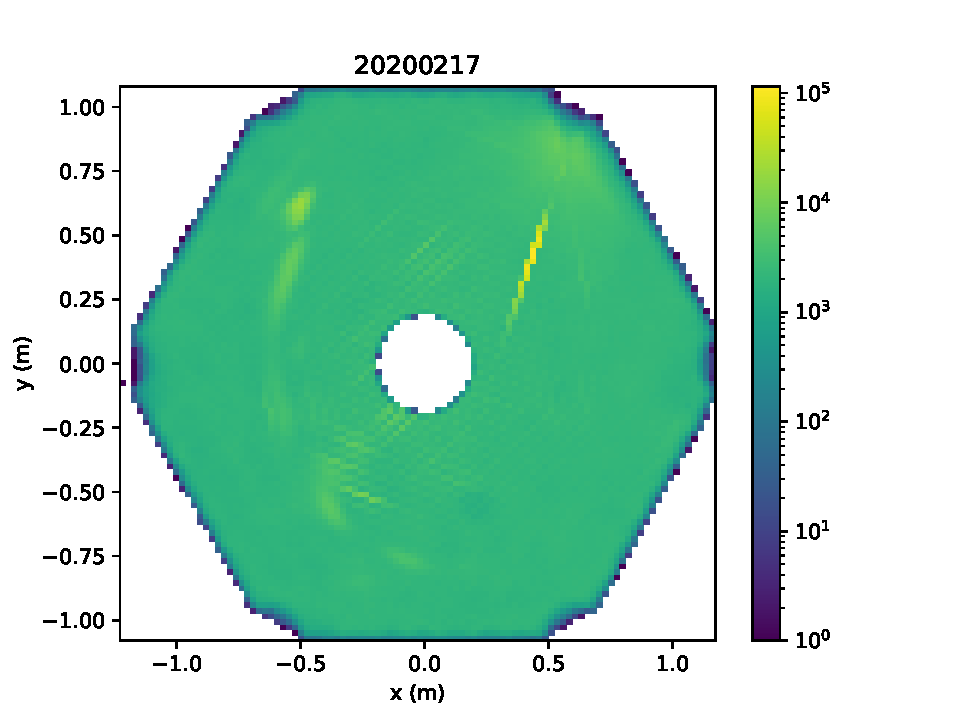
\includegraphics[width=\linewidth]{{Pictures/em_20200217_sizecut100}.pdf}
    \caption{\small 17/02/2020} \label{fig:3rd-cog-c}
  \end{subfigure}
  \begin{subfigure}{0.45\textwidth}
    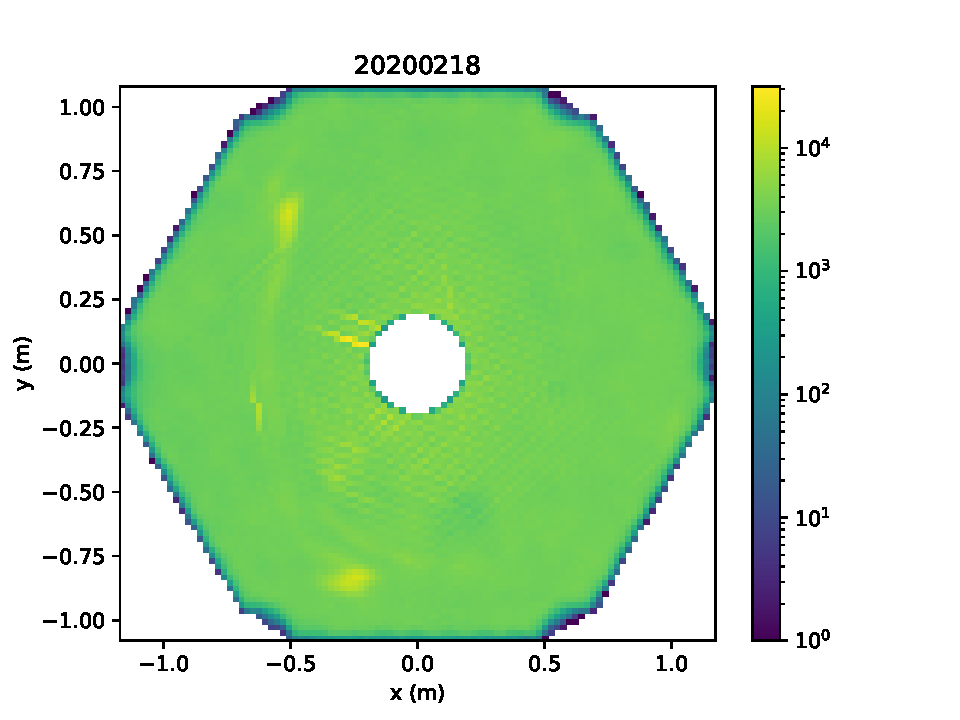
\includegraphics[width=\linewidth]{{Pictures/em_20200218_sizecut100}.pdf}
    \caption{\small 18/02/2020} \label{fig:3rd-cog-d}
  \end{subfigure} \\
  \begin{subfigure}{0.45\textwidth}
    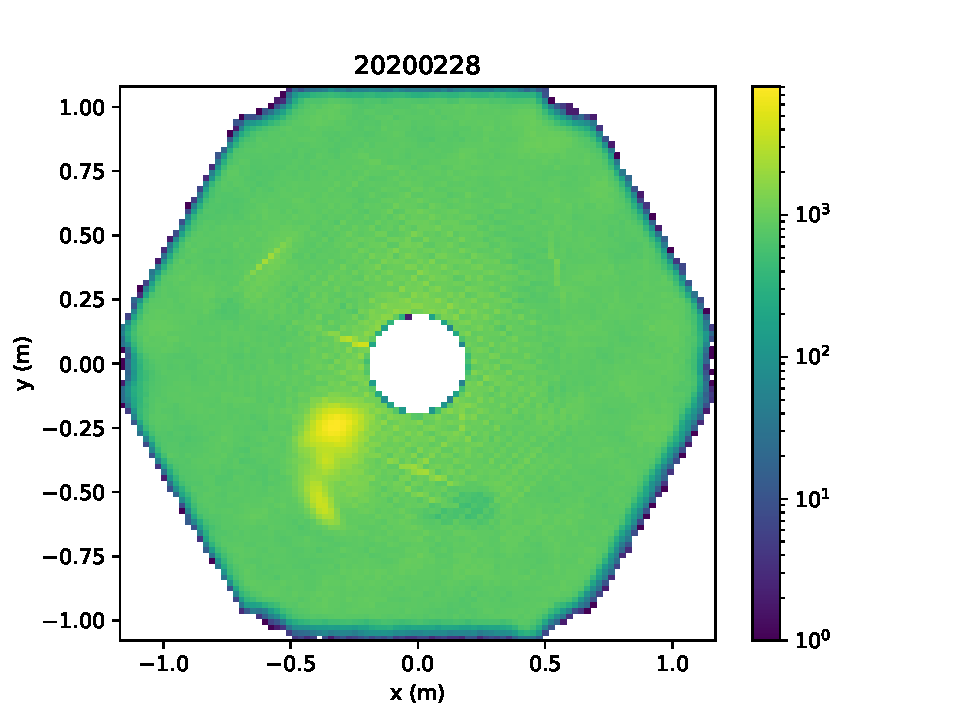
\includegraphics[width=\linewidth]{{Pictures/em_20200228_sizecut100}.pdf}
    \caption{\small 28/02/2020} \label{fig:3rd-cog-d}
  \end{subfigure}\\
  \caption{ Distribution of the positions in the camera of the center of gravity of Hillas ellipses for the data taken during the different days of the Third Crab Campaign, using the \gls{em} method for Hillas parameterization.\label{fig:em_3rd-crab-campaign-cog}}
\end{figure}



\end{document}
